\chapter{Discusión de resultados}
\label{ch:discusion-resultados}

\section{Toma de contacto}
bla

\section{Primera iteración}


% %* Comprobar
% \subsection{Módulo divisor de reloj}
% Distintas partes del circuito, trabajan a diferentes frecuencias, por tanto, se ha realizado un módulo que divida $n$ veces un reloj de entrada, tal que la frecuencia de salida sea $f_{out} = \frac{f_{in}}{2^n}$. Donde $n$ es el número de \emph{Flip-Flops} tipo D utilizados.
% En la figura~\ref{fig:clk_div_esquema} se muestra un ejemplo de funcionamiento.

% \begin{figure}[hbt]
%     \centering
%     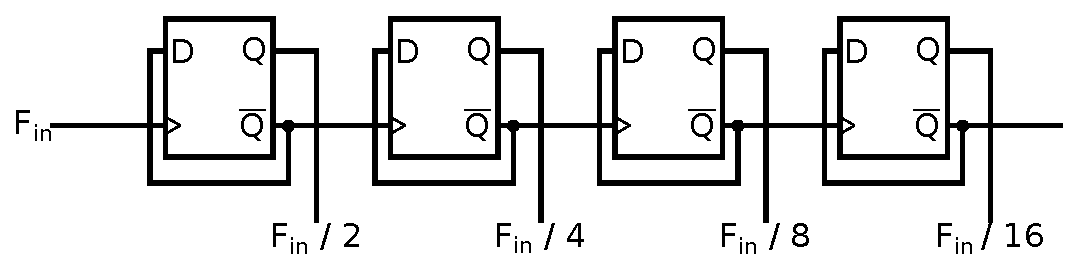
\includegraphics[width = 85mm]{esquemas/divisor_flipflop_D.eps}
%     \caption{Divisor de reloj con \emph{Flip-Flops}}
%     \label{fig:clk_div_esquema}
% \end{figure}

%! Revisar
\subsection{Módulo de envío datos por el puerto serie}
Debido a que la única forma de comunicación entre el PC y la \emph{FPGA} es a través de puerto serie, es necesario la realización de un módulo, genere y procese dichas señales. En esta priemra itraración de desarrollo, solo se diseño la funcionalidad básica de envío de datos, utilizada 

\subsection{Implementación básica ULPI}
\begin{itemize}
    \item No soporta la mayoría de funcionalidades deseadas.
    \item No se ha tenido en cuenta secuencia de inicio, por lo que había que hacerlo manualmente.
    \item Sin control de errores, por lo que había que reiniciar la FPGA cuando ocurriera uno.
\end{itemize}

\subsection{Reorientación}
Por una falta de metodología a seguir, y una implementación pobre del protocolo ULPI, se descarta todo lo anterior, y se empieza de nuevo de forma más ordenada, ciertas partes pueden ser reutilizadas posteriormente.

%!
\section{Segunda iteración}
%* Comprobar
En esta segunda iteración, y para evitar problemas futuros, se ha planteado una metodología de diseño y organización a seguir en todos los módulos. Dicha metodología, comentada con más detalle en el capítulo~\ref{ch:procedimiento}, se centra principalmente en organizar el código de una forma común, debiendo superar a su vez varias pruebas y simulaciones para poder ser utilizado.

%!
\subsection{Desarrollo de módulos principales}
% %! Revisar
% Ordenados cronologicamente
% Se desarrollan el resto de módulos necesarios (ver tarjeta "Estructurar las partes del sistema de captura", exceptuando signal\_trigger y btn\_debouncer). Ref anexos



\begin{itemize}
    %* Comprobar
    \item \textbf{Módulo divisor de reloj (clk\_div).} \\
    Módulo que divide un reloj de entrada, tal que la frecuencia de salida sea $f_{out} = \frac{f_{in}}{2^n}$, donde $n$ es el número de \emph{Flip-Flops} tipo D utilizados. En la figura~\ref{fig:clk_div_esquema} se muestra un ejemplo de funcionamiento.
    
    \begin{figure}[hbt]
        \centering
        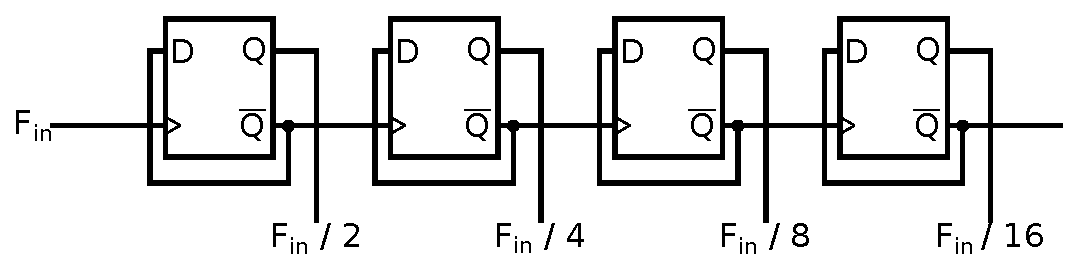
\includegraphics[width = 90mm]{esquemas/divisor_flipflop_D.eps}
        \caption{Divisor de reloj con \emph{Flip-Flops}}
        \label{fig:clk_div_esquema}
    \end{figure}

    A partir de él se generan dos relojes, uno basado en el reloj de $12MHz$ procedente de la placa \emph{iCEstick} (señal llamada clk\_div\_ice) y otro a partir del reloj de $60MHz$ del módulo USB3300 (señal  llamada clk\_div\_ULPI). Ambos relojes se dividen 24 veces y su única funcionalidad es la de  comprobar el funcionamiento del sistema por medio de los LEDs integrados en la placa.

    %! Revisar
    \item \textbf{Módulo de registro de desplazamiento universal.} \\
    Como se ha de desarrollar un módulo de comunicación serie, se ha diseñado un módulo que genere un registro de desplazamiento universal para facilitar la serialización y paralelización de los datos salientes y entrantes respectivamente. El módulo es capaz de producir tanto desplazamientos a derecha e izquierda de sus datos, como cargas y lecturas paralelas.

    \noWord[Añadir figura de capitulo objetivos???]

    %!
    \item \textbf{Módulo de generación de reloj de baudios.} \\
    De manera similar al módulo divisor de reloj, este genera un tren de pulsos a una frecuencia configurable, pero siendo la salida 

    %!
    \item \textbf{Módulo de comunicación serie.} \\
    Módulo de comunicación bidireccional entre el PC y la \emph{FPGA}, usado como canal por el que trasmitir los datos \emph{USB} capturados y recibir los comandos a ejecutar. Este módulo se ha dividido en otros tres, pudiendo facilitar su diseño.
    \begin{itemize}
        %!
        \item \textbf{Submódulo de recepción serie.} \\
        Está continuamente esperando a que la señal de entrada de datos serie (llamada \emph{UART\_Rx}) baje a un nivel bajo, a partir de cuando se activa

        \begin{figure}[hbt]
            \centering
            \begin{tikzpicture}[auto]
    % Config
    \tikzFlow

    % Place nodes
    \node [flowStart] (idle) {Reposo};
    
    \node [flowDecision] at ($ (idle)+(0,-2.65) $) (rxLow) {Entrada del puerto serie a nivel bajo?};
    
    \node [flowBase, below of=rxLow] (init) {Reinicio del contador de $bits$};
    
    \node [flowBase] at ($ (rxLow.east)+(3.85,1) $) (read) {Se guarda $bit$ entrante en el registro de desplazamiento};

    \node [flowDecision, below of=read] (10bitsDone) {Se han leído los $10~bits$ del mensaje?};
    
    \node [flowBase] at ($ (read)+(4.1,0) $) (increase) {Incremento del contador de $bits$};

    \node [flowBase] at ($ (10bitsDone)+(4.1,0) $) (wait) {Se espera un pulso del reloj de baudios};

    \node [flowBase, below of=10bitsDone] (save) {Se almacena el byte en memoria};

    % % Draw edges
    \path [flowLine] (idle) -- (rxLow);
    \path [flowLine] (rxLow) -- (init);
    \path [flowLine] (init.south) |- +(3.5,-1) |- (read.west);
    \path [flowLine] (read) -- (10bitsDone);
    \path [flowLine] (increase) -- (read);
    
    \node [flowHide] at ($ (idle)+(2.75,0) $) (anchor1) {};
    \path [flowLine] (rxLow) -- node [right, xshift=-1.2cm] {Sí} (init);
    \path [flowLine] (rxLow.east) node [above, xshift=0.2cm] {No} -| (anchor1.center);
    
    \path [flowLine] (save.east) -| +(4.5,0) |- (idle.east);
    
    \path [flowLine] (wait) -- (increase);
    \path [flowLine] (10bitsDone.east) node [above, xshift=0.2cm] {No} -- (wait);
    \path [flowLine] (10bitsDone) -- node [right, xshift=-1.2cm] {Sí} (save);
\end{tikzpicture}


% \begin{tikzpicture}[auto]
%     % Config
%     \tikzFlow

%     % Place nodes
%     \node [flowStart] (idle) {Reposo};
    
%     \node [flowDecision, below of=idle] (rxLow) {Entrada del puerto serie a nivel bajo?};
    
%     \node [flowBase, below of=rxLow] (init) {Reinicio del contador de $bits$};
    
%     \node [flowBase, below of=init] (read) {Se guarda $bit$ entrante en el registro de desplazamiento};

%     \node [flowDecision, below of=read] (10bitsDone) {Se han leído los $10~bits$ del mensaje?};
    
%     \node [flowBase] at ($ (read)+(4.1,0) $) (increase) {Incremento del contador de $bits$};

%     \node [flowBase] at ($ (10bitsDone)+(4.1,0) $) (wait) {Se espera un pulso del reloj de baudios};

%     \node [flowBase, below of=10bitsDone] (save) {Se almacena el byte en memoria};

%     % % Draw edges
%     \path [flowLine] (idle) -- (rxLow);
%     \path [flowLine] (rxLow) -- (init);
%     \path [flowLine] (init) -- (read);
%     \path [flowLine] (read) -- (10bitsDone);
%     \path [flowLine] (increase) -- (read);
    
%     \node [flowHide] at ($ (idle)+(3.5,0) $) (anchor1) {};
%     \path [flowLine] (rxLow) -- node [right, xshift=-1.2cm] {Sí} (init);
%     \path [flowLine] (rxLow.east) -| node [above, xshift=-1.2cm] {No} (anchor1.center);
    
%     \path [flowLine] (save.east) -| +(4.5,0) |- (idle.east);
    
%     \path [flowLine] (wait) -- (increase);
%     \path [flowLine] (10bitsDone.east) node [above, xshift=0.2cm] {No} -- (wait);
%     \path [flowLine] (10bitsDone) -- node [right, xshift=-1.2cm] {Sí} (save);
% \end{tikzpicture}
            \caption{Diagrama de funcionamiento del submódulo de recepción serie}
            \label{fig:flujo_uart_rx}
        \end{figure}

        %!
        \item \textbf{Submódulo de emisión serie.} \\
        a
        
        %!
        \item \textbf{Submódulo de uni'o.} \\
        
    \end{itemize}
    
    %!
    \item \textbf{Módulo de comunicación \emph{ULPI}.} \\
    \begin{itemize}
        %!
        \item \textbf{Submódulo de escritura de registros serie.} \\
        a

        %!
        \item \textbf{Submódulo de emisión serie.} \\
        a
        
        %!
        \item \textbf{Submódulo general.} \\
        a
    \end{itemize}
    
    %!
    \item \textbf{Módulo de memoria \emph{FIFO}.} \\
    \begin{itemize}
        %!
        \item \textbf{FIFO\_BRAM\_SYNC\_CUSTOM} \\
        a

        %!
        \item \textbf{FIFO\_BRAM\_SYNC} \\
        a
    \end{itemize}
    
    %!
    \item \textbf{Implementación FIFO en UART.} \\
    a
    
    %!
    \item \textbf{Módulo que obtenga y almacene los comandos desde el PC.} \\
    a
    
    %!
    \item \textbf{Botones.} \\
    a
    
    %!
    \item \textbf{Controlador.} \\
    a
    
    %!
    \item \textbf{Top.} \\
    a
\end{itemize}

\subsection{Pieza 3D}
Para poder trabajar de forma más fluida y con menor probabilidad de ruptura accidental, se ha diseñado e impreso una simple pieza 3D en la que situar todas las partes (IceStick + USB3300).

\subsection{Botonera externa}
Se agrega botonera externa que permita resetar el sistema sin tener que desconectar y enviar byte de prueba.

\subsection{Errores con Yosys}
\begin{itemize}
    \item Errores puerta triestato. \\
    Incluso habiendo realizado una prueba para comprobar el funcionamiento de entradas triestato, siendo esta positiva, al realizar una prueba con el módulo de ULPI, yosys daba errores, y pedía que instanciara los puertos de entrada y salida manualmente para que funcionase. Tras buscar información en diversas fuentes y conseguir una correcta instanciacion de los puertos de entrada, se puede continuar sin problemas. ACTUALIZACION Este error ha sido ya solucionado por parte de Yosys, por lo que es suficiente el utilizar una asignación triestato.

    \item Error sintetizacion \\
    Las últimas versiones de yosys lanzan un error desconocido al intentar sintetizar, por lo que por el momento, se utiliza una versión anterior. ACTUALIZACION Ya funciona cambiando varios bits de los modulos de memoria FIFO.
\end{itemize}

\subsection{Mis errores destacables}
\begin{itemize}
    \item Error inicialización FIFO \\
    Error al diseñar el modulo FIFO. Instanciaba los modulos de memoria de forma incorrecta, utilizaba los 8 primeros bits, pero en realidad el módulo utiliza (para el caso de 8bits) los bits pares. Este error producia perdida de información.
    
    \item Mis errores más destacables \\
    Error al poner el bus ULPI en el archivo principal como input (solo entrada) en vez de inout (bidireccional).
\end{itemize}


\section{Procesado de datos obtenidos}

\subsection{Comandos disponibles}
Una vez ya con la parte "hardware" lista, se empieza con la parte "software". Los datos capturados vienen por el puerto serie utilizando un protocolo básico, con 4 posibles comandos por parte del PC.
\begin{itemize}
    \item Leer registro.
    \item Escribir registro.
    \item Enviar al PC valor leído del registro.
    \item Activar/desactivar envío de datos USB.
\end{itemize}

\subsection{Menú de control}
Se escribe un pequeño menú de control (menu.c y menu.h). Con el se puede configurar el puerto serie, la velocidad, abrir/cerrar puerto, realizar los 4 comandos anteriores y salir.

\subsection{Libreria libserialport}
Se utiliza la libreria libserialport (\href{https://sigrok.org/wiki/Libserialport}) para trabajar con el puerto serie.

\subsection{Librería de control serie}
Se escribe la librería de control serie [serial\_ctrl] (serial\_ctrl.h y serial\_ctrl.c), con ella se crean varias estructuras de control y se añaden varias funciones que controlen varias acciones del puerto serie (init, etc..) y de los comandos.

\subsection{Hilos}
Como el menú está continuamente esperando una entrada del usuario, se crean dos hilos distintos, uno para el control del menú, y otro para gestionar las acciones. Poseen un "semaforo" rudimentario para sincronizarse mutuamente. Las funciones de ambos hilos están programadas en thread\_functions (thread\_functions.h y thread\_functions.c).
\begin{itemize}
    \item menu\_thread\_loop. \\
    Bucle que se encarga de controlar el menu.

    \item serial\_thread\_loop. \\
    Bucle que se encarga de todas las funciones relacionadas con el puerto serie, acciones provenientes de menu\_thread\_loop.
\end{itemize}

\subsection{Almacenaje de datos}
    



% Comentatrios de los problemas encontrados y/o dificultad de depurar en la FPGA

\noWord[Detalles de los modulos, diagrams de flujo, etc...]

% \chapter{Discusión de resultados}
% \label{ch:discusion-resultados_plantilla}

% La discusión de resultados se presenta de forma separada a los resultados propiamente dichos, porque de esta forma los resultados son directamente aprovechables en cualquier trabajo derivado.  Pero si el capítulo queda demasiado pequeño no dudes en mezclarlo con el anterior en un único capítulo de \emph{Resultados y discusión} o con el siguiente en un capítulo de \emph{Discusión de resultados y conclusiones}.